\section{Partitioning for Spark}
%$$$$$$$$$$$$$$$$$$$$$$$$$$$$$$$$$$$$$$$$$$$$$$$$$$$$$$$$$$$$$$$$$$$$$$$$$$$$$$$$
%$$$$$$$$$$$$$$$$$$$$$$$$$$$$$$$$$$$$$$$$$$$$$$$$$$$$$$$$$$$$$$$$$$$$$$$$$$$$$$$$
% 일반적인 매니코어 또는 Scale-server의 scalability 대한 설명과 이번장에 대한 설명
%$$$$$$$$$$$$$$$$$$$$$$$$$$$$$$$$$$$$$$$$$$$$$$$$$$$$$$$$$$$$$$$$$$$$$$$$$$$$$$$$
\ifkor
파티션닝 방법이 필요한 이유는 spark library와 runtime엔진이 single node에 동작하는 
시스템의 scalability 특성을 고려하지 않았기 때문이다. 
scale-up server를 위한 spark scalability의 근본적인 해결 방법은 spark library와 
runtime엔진을 scale-up서버를 위해 scalable하게 만드는 것이다.
하지만 scale-out 시스템의 scalability를 위해 작성된 spark의 library와 runtime 엔진을 
수정하는것은 쉽지않다.
이러한 single node로 구성된 manycore scale-up 서버에 대한 scalability
문제는 도커를 활용한 파티셔닝 기법을 사용하여 해결할 수 있다.
이번 장에서는 우리가 수행한 파티션닝 방법이 필요한 이유와 우리가 수행한 방법에 대해서 설명한다.
\else

\fi

%$$$$$$$$$$$$$$$$$$$$$$$$$$$$$$$$$$$$$$$$$$$$$$$$$$$$$$$$$$$$$$$$$$$$$$$$$$$$$$$$
%$$$$$$$$$$$$$$$$$$$$$$$$$$$$$$$$$$$$$$$$$$$$$$$$$$$$$$$$$$$$$$$$$$$$$$$$$$$$$$$$
% NUMA 영향에 대한 설명
%$$$$$$$$$$$$$$$$$$$$$$$$$$$$$$$$$$$$$$$$$$$$$$$$$$$$$$$$$$$$$$$$$$$$$$$$$$$$$$$$
\ifkor
파티션닝 방법이 필요한 가장 큰 이유는 DRAM access latency 때문이다. 
만약 scale-up server가 NUMA 아키텍쳐를 가진 경우일 경우, 
리눅스는 이러한 문제를 해결하기 위해 커널 내부에 automatic NUMA balancing이라는 기능이 있으나, 
아직 파티션되어 수행하는 방법보다는 성능이 떨어진다[]. 그림 xx-xx는 NUMA balancing을 
사용한 방법과 파티션기법을 사용한 방법의 성능 측정한 결과를 보여준다. 
\else

\fi

%$$$$$$$$$$$$$$$$$$$$$$$$$$$$$$$$$$$$$$$$$$$$$$$$$$$$$$$$$$$$$$$$$$$$$$$$$$$$$$$$
%$$$$$$$$$$$$$$$$$$$$$$$$$$$$$$$$$$$$$$$$$$$$$$$$$$$$$$$$$$$$$$$$$$$$$$$$$$$$$$$$
% Linux kernel scalability (lock, cache cohearnci, scheduler)등등 OS 노이즈에 대한 설명
%$$$$$$$$$$$$$$$$$$$$$$$$$$$$$$$$$$$$$$$$$$$$$$$$$$$$$$$$$$$$$$$$$$$$$$$$$$$$$$$$
\ifkor
NUMA의 영향 뿐만 아니라, operating system의 scalability 저해 요소 때문에 파티션닝 방법은 필요하다.
Shared memory 시스템의 공유데이터 때문에 발생하는 scalability 저해 요소 때문에 필요하다.
첫째로 공유 데이터를 lock이 있다. 표 xxx 앞에서 실험한 spark의 wordcount에 대해서 .
JVM 위에서 동작하는 thread간의 공유하는 single address space때문에 발생하는 공유 문제이다.
다음으로 scheduler가 아직 
마지막으로 cache cohearci traffic이 있다. 

\else

\fi

%$$$$$$$$$$$$$$$$$$$$$$$$$$$$$$$$$$$$$$$$$$$$$$$$$$$$$$$$$$$$$$$$$$$$$$$$$$$$$$$$
%$$$$$$$$$$$$$$$$$$$$$$$$$$$$$$$$$$$$$$$$$$$$$$$$$$$$$$$$$$$$$$$$$$$$$$$$$$$$$$$$
% 스파크는 결국 : shared memory system -> distributed system 처럼해야한다. 
%$$$$$$$$$$$$$$$$$$$$$$$$$$$$$$$$$$$$$$$$$$$$$$$$$$$$$$$$$$$$$$$$$$$$$$$$$$$$$$$$
\ifkor
이처럼 NUMA와 shared memory의 공유 데이터 때문에 발생하는 scalability 저해 요소 때문에, 
scale-up 서버를 위한 스파크도 distributed system의 개념처럼 동작해야한다.
따라서 본 연구는 메모리와 CPU를 파티션닝을 하여 마치 shared memory 시스템을 distributed system 
처럼 동작하도록 제안 한다.
스마크 워커들은 모두 독립적인 cpu와 memory를 할당받아 최대한 thread간의 공유메모리와 remote
memory에 접근을 막도록 하였다.
\else

\fi

\begin{figure}[h]
  \begin{center}
     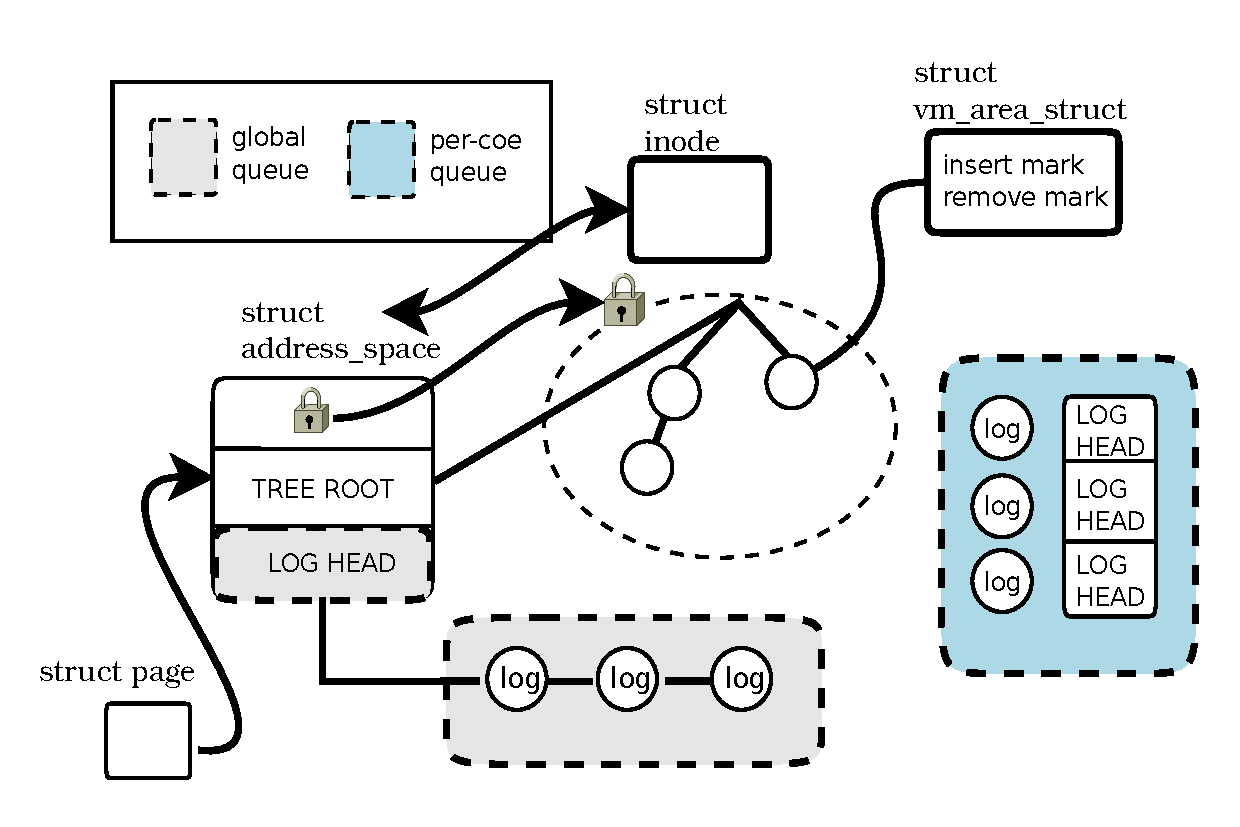
\includegraphics[width=0.5\textwidth]{fig/jaildocker}
  \end{center}
  \caption{The example showing seven update operations(insert C, insert D ,
  reader executes with lock.}
  \label{fig:basic}
\end{figure}


%$$$$$$$$$$$$$$$$$$$$$$$$$$$$$$$$$$$$$$$$$$$$$$$$$$$$$$$$$$$$$$$$$$$$$$$$$$$$$$$$
%$$$$$$$$$$$$$$$$$$$$$$$$$$$$$$$$$$$$$$$$$$$$$$$$$$$$$$$$$$$$$$$$$$$$$$$$$$$$$$$$
% 제안하는 구조 framework 설명
%$$$$$$$$$$$$$$$$$$$$$$$$$$$$$$$$$$$$$$$$$$$$$$$$$$$$$$$$$$$$$$$$$$$$$$$$$$$$$$$$
\ifkor
본 연구에서 제안하는 구조는 그림 <x>와 같다. 
모든 cpu들은 파티션이 되어 동작하며, 모두 스파크 워커로 동작한다.
도커의 파티션은 한 소켓에서 해당하는 cpu 수를 최대로 하여 파티션을 한 후 
계속 코어 수를 줄이며 파티션을 수행한다. 
예를 들어 15코어를 가진 NUMA 노드일 경우, 15코어 단위로 Docker 파티션을 구성 한 후,
(7,8) 와 같이 추가적인 파티션 조합으로 구성한다.
이러한 파티션은 
가장 최적의 방법은 best fit을 찾는 과정이 필요하다. 
\else

\fi


%$$$$$$$$$$$$$$$$$$$$$$$$$$$$$$$$$$$$$$$$$$$$$$$$$$$$$$$$$$$$$$$$$$$$$$$$$$$$$$$$
%$$$$$$$$$$$$$$$$$$$$$$$$$$$$$$$$$$$$$$$$$$$$$$$$$$$$$$$$$$$$$$$$$$$$$$$$$$$$$$$$
% Docker를 이용하는 이유
%$$$$$$$$$$$$$$$$$$$$$$$$$$$$$$$$$$$$$$$$$$$$$$$$$$$$$$$$$$$$$$$$$$$$$$$$$$$$$$$$
\ifkor
우리는 Worker들의 파티션닝을 위해 Docker container를 사용하였다. 
그 이유는 virtual machine보다 훨씬 가벼운 구조로 되어 있으며, 
최근 docker기반으로 시스템을 관리하는 구조로 변경되고 있기 때문이다.
예를 들어 google kubernet을 사용할 경우, 워크마다 가장 최적의 파티션닝 값을 구한 후
그에 맞는 도커 컨테이너를 실행시키는 방법으로 구성하면 된다.
따라서 본 연구의 파티셔닝을 위한 방법으로 Docker container를 사용하였다.
\else

\fi


The basic principle of update-side absorbing is that update uses atomic 
marking operation for the object's mark field, which allows previous operation to cancel.
For instance, if a new remove operation occurs after insert operation of the
same object, deferu does not store this operation in the lock-less
list; instead, it changes the insert mark field to zero using the CAS.
This mark is checked later when reading operation occurs and the operation log 
maintained in the lock-less list is applied to original data structure atomically.




%$$$$$$$$$$$$$$$$$$$$$$$$$$$$$$$$$$$$$$$$$$$$$$$$$$$$$$$$$$$$$$$$$$$$$$$$$$$$$$$$
%$$$$$$$$$$$$$$$$$$$$$$$$$$$$$$$$$$$$$$$$$$$$$$$$$$$$$$$$$$$$$$$$$$$$$$$$$$$$$$$$
% Linux kernel scalability (lock, cache cohearnci, scheduler)등등 OS 노이즈에 대한 설명
%$$$$$$$$$$$$$$$$$$$$$$$$$$$$$$$$$$$$$$$$$$$$$$$$$$$$$$$$$$$$$$$$$$$$$$$$$$$$$$$$
\ifkor
NUMA의 영향 뿐만 아니라, operating system의 scalability 저해 요소 때문에 파티션닝 방법은 필요하다.
Shared memory 시스템의 공유데이터 때문에 발생하는 scalability 저해 요소 때문에 필요하다.
첫째로 공유 데이터를 lock이 있다. 표 xxx 앞에서 실험한 spark의 wordcount에 대해서 .
JVM 위에서 동작하는 thread간의 공유하는 single address space때문에 발생하는 공유 문제이다.
다음으로 scheduler가 아직 
마지막으로 cache cohearci traffic이 있다. 

\else

\fi


